\section{Materials}
\label{sec:chp3-sec3}
This section describes the dermosopy datasets, used in our experiments.
The primary tests were conducted based on the Vienna dataset~\cite{ganster2001automated}, which we had access to thanks to Dr. H.~Ganster.
However, later, due to confidentiality problems, our access to this dataset was limited and we chose to work with PH$^{2}$~\cite{mendoncca2013ph}, the only publicly available dermoscopy dataset.
%Figures~\ref{fig:Viennasamples} and~\ref{fig:PH2samples} demonstrate the variation of colors between each lesion and similar color characteristics in melanoma, dysplastic and benign lesions found in the two datasets.
The remainder of this section details these datasets while a summary is listed in Table~\ref{tab:tableDataset}.


\begin{table}[H]
\caption{Summary of Vienna and PH$^{2}$ Datasets. M, D, and B stand for melanoma, dysplastic and benign samples, respectively.}
\centering
\resizebox{0.9\linewidth}{!}{
\begin{tabular}{l c c c c c c c c}
\toprule
Dataset & \# samples & \# M & \# D & \# B & Resolution $\si{px}$ & Released & Public & Segmentation \\
\midrule
Vienna & 5380 & 101 & 1002 & 4277 & $632 \times 387 $ & 2001 & - & - \\
PH$^{2}$ & 200 & 40 & 80 & 80 & $768 \times 560$ & 2013 & $\checkmark$ & $\checkmark$ \\
\bottomrule
\end{tabular}}
\label{tab:tableDataset}
\end{table}

\begin{description}
\item [The Vienna dermoscopy dataset] was acquired by the \textit{Department of Dermatology at the Vienna General Hospital, Austria}.
The images were captured using a hand-held CCD camera equipped with an epiluminescence microscope~\cite{ganster2001automated}.
The acquired  true-color 8-bit RGB images have a resolution of 632$\times$3871 pixels (1 pixel $\approx$ 22 \si{\micro\metre}$^{2}$) and were recorded without any color normalization.
This is a large-scale dataset (group~5) with over 5000 lesions including 4277 benign, 1002 dysplastic and 101 malignant melanoma lesions.
In this dataset, the dysplastic and melanoma lesions were surgically removed and their ground truth diagnosis were provided by histological analysis~\cite{ganster2001automated}. 
This dataset was also used in \cite{torre2010learning,maglogiannis2009overview}. 
Figure.~\ref{fig:Viennasamples} shows three sample images from this dataset, one for each class.
The images in this dataset were acquired under different conditions and are illumination imbalanced.
\begin{figure}
\begin{center}
  \hspace*{\fill}
  \subfloat[Melanoma lesion]{
    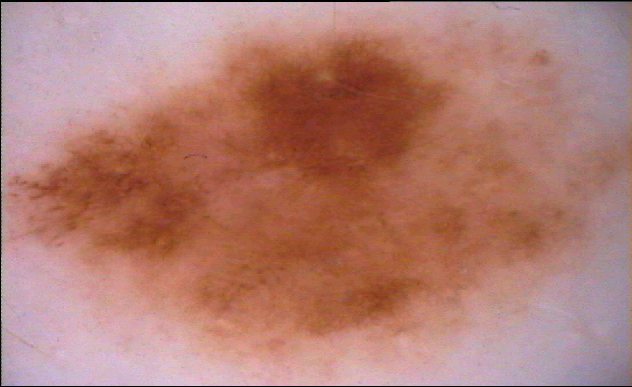
\includegraphics[width=0.32\textwidth]{Chapter3/Figures/M2_Vienna.png}}\hfill
  \subfloat[Dysplastic lesion]{
    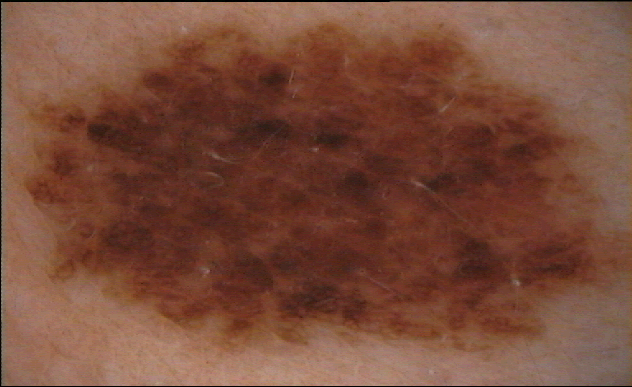
\includegraphics[width=0.32\textwidth]{Chapter3/Figures/D1_Vienna.png}}\hfill
  \subfloat[Benign lesion]{
    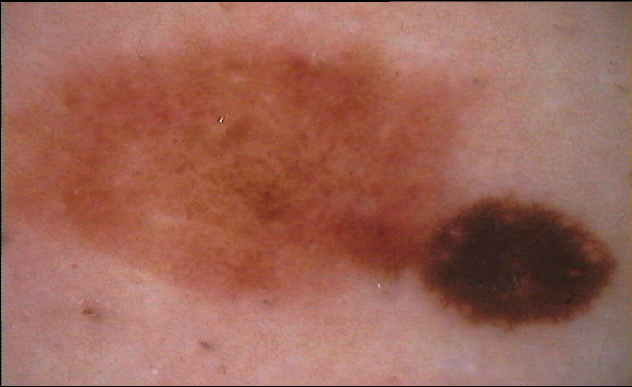
\includegraphics[width=0.32\textwidth]{Chapter3/Figures/B2_Vienna.png}}
  \hspace*{\fill}
  \caption[Sample images of the Vienna dataset]{Sample images for the Vienna dataset depicting (a) melanoma, (b) dysplastic and (c) benign lesions.}
  \label{fig:Viennasamples}
\end{center}	
\end{figure}

\item [The PH$^{2}$ dataset] was acquired at the \textit{Dermatology Service of the Hospital Pedro Hispano, Matosinhos, Portugal}~\cite{mendoncca2013ph} with the Tuebinger Mole Analyzer system using a magnification of $20\times$.
The 8-bits~RGB color dermoscopic images were obtained under the same conditions with a resolution of 768$\times$560 pixels. 
This dataset contains 200 dermoscopic images divided into 160 benign/dysplastic and 40 melanoma lesions. 
The lesions are segmented and their histological diagnosis are provided as the ground-truth. 
Figure~\ref{fig:PH2samples} shows three image samples from this dataset, representing melanoma, dysplastic, and benign lesions. 
\begin{figure}
\begin{center}
  \hspace*{\fill}
  \subfloat[Melanoma lesion]{
    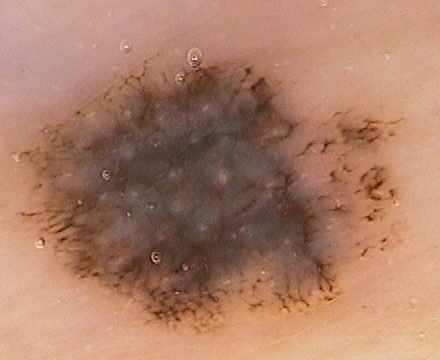
\includegraphics[width=0.32\textwidth, height= 0.18\textheight]{Chapter3/Figures/M1_PH2.png}}\hfill
  \subfloat[Dysplastic lesion]{
    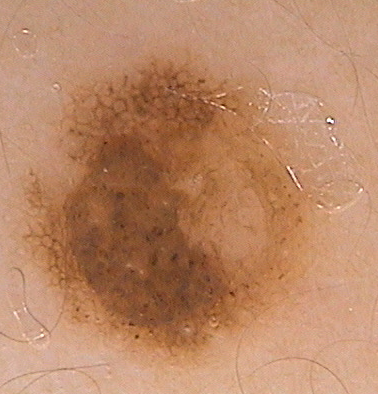
\includegraphics[width=0.32\textwidth, height= 0.18\textheight]{Chapter3/Figures/D1_PH2.png}}\hfill
  \subfloat[Benign lesion]{
    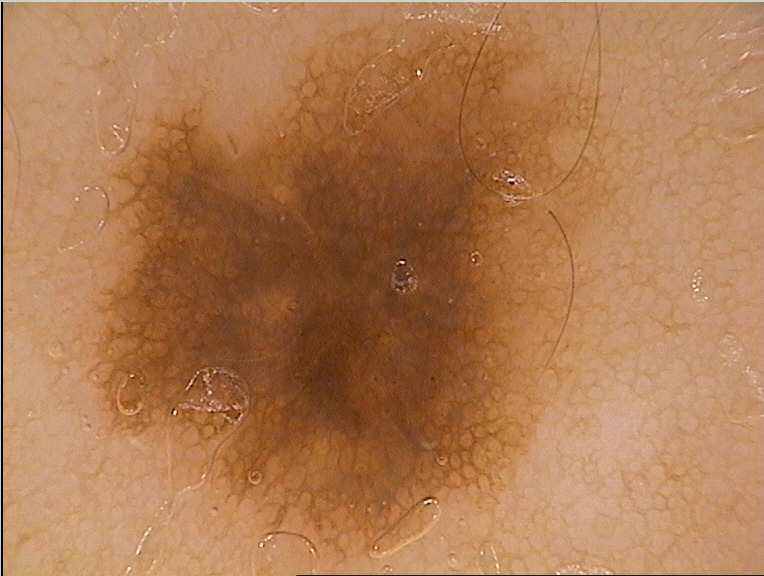
\includegraphics[width=0.32\textwidth, height= 0.18\textheight]{Chapter3/Figures/B1_PH2.png}}
  \hspace*{\fill}
  \caption[Image samples of the PH$^{2}$ dataset]{Image samples for the PH$^2$ dataset depicting (a) melanoma, (b) dysplastic and (c) benign lesions.}
  \label{fig:PH2samples}
\end{center}	
\end{figure}

\end{description}
Both figures~\ref{fig:Viennasamples} and~\ref{fig:PH2samples} show the variation of colors between each lesion and similar color characteristics between melanoma, dysplastic and benign lesions.

	%\
%%% Local Variables: 
%%% mode: latex
%%% TeX-master: "../thesis"
%%% End: 
